\section{Methods}

All experiments were approved by the Champalimaud Foundation Bioethics Committee and the Portuguese National Authority for Animal Health, Direcção\hyp{}Geral de Alimentação e Veterinária (DGAV).

\textbf{Lesions:} Ibotenic acid was injected bilaterally in 11 Long-Evans rats (ages from 83 to 141 days; 9 females, 2 males), at 3 injection sites with 2 depths per site (\SI{-1.5}{\milli\meter} and \SI{-0.75}{\milli\meter} from the surface of the brain). At each depth we injected a total amount of \SI{82.8}{\nano\liter} using a microinjector (Drummond Nanoject II, \SI{9.2}{\nano\liter} per injection, 9 injections per depth). The coordinates for each site, in \si{\milli\meter} with respect to Bregma, were: +1.0 AP / 2.0 ML; +1.0 AP / 4.0 ML; +3.0 AP / 2.0 ML, following the protocol reported by Kawai et al. for targeting forelimb motor cortex \cite{Kawai2015}. Five other animals were used as sham controls (age-matched controls; 3 females, 2 males), subject to the same intervention, but where ibotenic acid was replaced with physiological saline. Six additional animals were used as wildtype, no-surgery, controls (age-matched controls; 6 females).

For the frontal cortex aspiration lesions, the margins of the craniotomy were extended to cover from -2.0 to +5.0 \si{\milli\meter} AP relative to Bregma and laterally from 0.5 \si{\milli\meter} up to the temporal ridge of the skull. After removal of the skull, the exposed dura was cut and removed, and the underlying tissue aspirated to a depth of 2 to 3 \si{\milli\meter} with a fine pipette \cite{Whishaw2000}. For the frontoparietal cortical lesions, the craniotomy extended from -6.0 to +4.0 \si{\milli\meter} AP relative to Bregma and laterally from 0.5 \si{\milli\meter} up to the temporal ridge. Two of these animals underwent aspiration lesions as described above. In the remaining animal, the lesion was induced by pial stripping in order to further restrict the damage to cortical areas. After removal of the dura, the underlying pia, arachnoid and vasculature were wiped with a sterile cotton swab until no vasculature was visible \cite{Farr2002}.

\textbf{Recovery period:} After the surgeries, animals were given a minimum of one week (up to two weeks) recovery period in isolation. After this period, animals were handled every day for a week, after which they were paired again with their age-matched control to allow for social interaction during the remainder of the recovery period. In total, all animals were allowed at least one full month of recovery before they were first exposed to the behaviour assay.

The three largest frontoparietal lesioned animals were originally prepared for a study of behaviour in a dynamic visual foraging task, which they were exposed to for one month in addition to the recovery period described above. This task did not, however, require any challenging motor behaviours besides locomotion over a completely flat surface. This period was also used to monitor the overall health condition of the animals and to facilitate sensorimotor recovery as much as possible. The animal with the largest lesion (Extended Lesion F) was prevented from completing the behaviour protocol due to deteriorating health conditions following the first two days of testing.

\textbf{Histology:} All animals were perfused intracardially with 4\% paraformal\-dehyde in phosphate buffer saline (PBS) and brains were post-fixed for at least \SI{24}{\hour} in the same fixative. Serial coronal sections (\SI{100}{\micro\meter}) were Nissl-stained and imaged for identification of lesion boundaries. In two of the largest frontoparietal lesions (Extended Lesions D and E), serial sections were taken sagittally.

In order to reconstruct lesion volumes, the images of coronal sections were aligned and the outlines of both brain and lesions were manually traced in Fiji \cite{Schindelin2012} and stored as two-dimensional regions of interest. Lesion volumes were calculated by summing the area of each region of interest multiplied by the thickness of each slice. The stored regions were also used to reconstruct a 3D polygon mesh for visualization of lesion boundaries.

\textbf{Behaviour assay:} During each session the animal was placed inside a behaviour box for \SI{30}{\minute}, where it could collect water rewards by shuttling back and forth between two nose pokes (Island Motion Corporation, USA). To do this, animals had to cross a \SI{48}{\centi\meter} obstacle course composed of eight \SI{2}{\centi\meter} aluminium steps spaced by \SI{4}{\centi\meter} (Figure \ref{fig:shuttlingProtocol}). The structure of the assay and each step in the obstacle course was built out of aluminium structural framing (Bosch Rexroth, DE, \SI{20}{\milli\meter} series). The walls of the arena were fabricated with a laser-cutter from \SI{5}{\milli\meter} thick opaque black acrylic and fixed to the structural framing. A transparent acrylic window partition was positioned in front of the obstacle course in order to provide a clear view of the animal. All experiments were run in the dark by having the behavioural apparatus enclosed in a light tight box.

\begin{figure}
\begin{center}
\includesvg[width=\columnwidth]{chapters/figuresChBehaviour/shuttlingProtocol}
\end{center}
\vspace{-5mm}
\caption{Schematic of the apparatus and summary of the different conditions in the shuttling protocol.}
\label{fig:shuttlingProtocol}
\end{figure}

A motorized brake allowed us to lock or release each step in the obstacle course (Figure \ref{fig:shuttlingSteps}). The shaft of each of the obstacles was coupled to an acrylic piece used to control the rotational stability of each step. In order to lock a step in a fixed position, two servo motors are actuated to press against the acrylic piece and hold it in place. Two other acrylic pieces were used as stops to ensure a maximum rotation angle of approximately +/- \ang{100}. Two small nuts were attached to the bottom of each step to work as a counterweight that gives the obstacles a tendency to return to their original flat configuration. In order to ensure that noise from servo motor actuation could not be used as a cue to tell the animal about the state of each step, the motors were always set to press against an acrylic piece, either the piece that keeps the step stabilized, or the acrylic stops. At the beginning of each trial, the motors were run through a randomized sequence of positions in order to mask information about state transitions and also to ensure the steps were reset to their original configuration. Control of the motors was done using a Motoruino board (Artica, PT) along with a custom workflow written in the Bonsai visual programming language \cite{Lopes2015a}.

\begin{figure}
\begin{center}
\includesvg[width=0.5\columnwidth]{chapters/figuresChBehaviour/shuttlingSteps}
\end{center}
\vspace{-5mm}
\caption{Schematic of the step locking mechanism and load cell sensor.}
\label{fig:shuttlingSteps}
\end{figure}

\textbf{Data acquisition:} The behaviour of the animals was recorded with a high-speed and high-resolution videography system (1280x680 @ \SI{120}{\hertz}) using an infrared camera (Flea3, PointGrey, CA), super-bright infrared LED front lights (SMD5050, 850 nm) and a vari-focal lens (Fujinon, JP) positioned in front of the transparent window partition. A top view of the assay was simultaneously recorded with the same system at a lower frame-rate (\SI{30}{\hertz}) for monitoring purposes. All video data was encoded with MPEG-4 compression for subsequent offline analysis. Behaviour data acquisition for the nose poke beam breaks was done using an Arduino board (Uno, Arduino, USA) and streamed to the computer via USB. All video and sensor data acquisition was recorded in parallel using the same Bonsai workflow used to control the behaviour assay.

\textbf{Behaviour protocol:} The animals were kept in a state of water deprivation for \SI{20}{\hour} prior to each daily session. For every trial, rats were delivered a \SI{20}{\micro\liter} drop of water. At the end of each day, they were given free access to water for \SI{10}{\minute} before initiating the next deprivation period. Sessions lasted for six days of the week from Monday to Saturday, with a day of free access to water on Sunday. Before the start of the water deprivation protocol, animals were run on a single habituation session where they were placed in the box for a period of \SI{15}{\minute}.

The following sequence of conditions were presented to the animals over the course of a month (see also Figure \ref{fig:shuttlingProtocol}): day 0, habituation to the box; day 1-4, all the steps were fixed in a stable configuration; day 5, 20 trials of the stable configuration, after which the two center steps were made unstable (i.e. free to rotate); day 6-10, the center two steps remained unstable; day 11, 20 trials of the unstable configuration, after which the two center steps were again fixed in a stable state; day 12, all the steps were fixed in a stable configuration; day 13-16, the state of the center two steps was randomized on a trial-by-trial basis to be either stable or unstable. Following the end of the random protocol, animals continued to be tested in the assay for a variable number of days (up to one week) in different conditions. At the end of the testing period, all animals were exposed to a final session where all steps were made free to rotate in order to assay locomotion performance under challenging conditions.

\textbf{Data analysis:} All scripts and custom code used for data analysis are available online\footnote{https://bitbucket.org/kampff-lab/shuttling-analysis}. The raw video data was first pre-processed using a custom Bonsai workflow in order to extract features of interest (Figure \ref{fig:videography}). Tracking of the nose was achieved by background subtraction and connected component labelling of segmented image elements. First we compute the ellipse best-fit to the largest object in the image. We then mark the tip of the nose as the furthermost point, in the segmented shape of the animal, along the major axis of the ellipse. In order to analyse stepping performance, regions of interest were defined around the surface of each step and in the gaps between the steps. Background subtracted activity over these regions was recorded for every frame for subsequent detection and classification of steps and slips.

\begin{figure}
\begin{center}
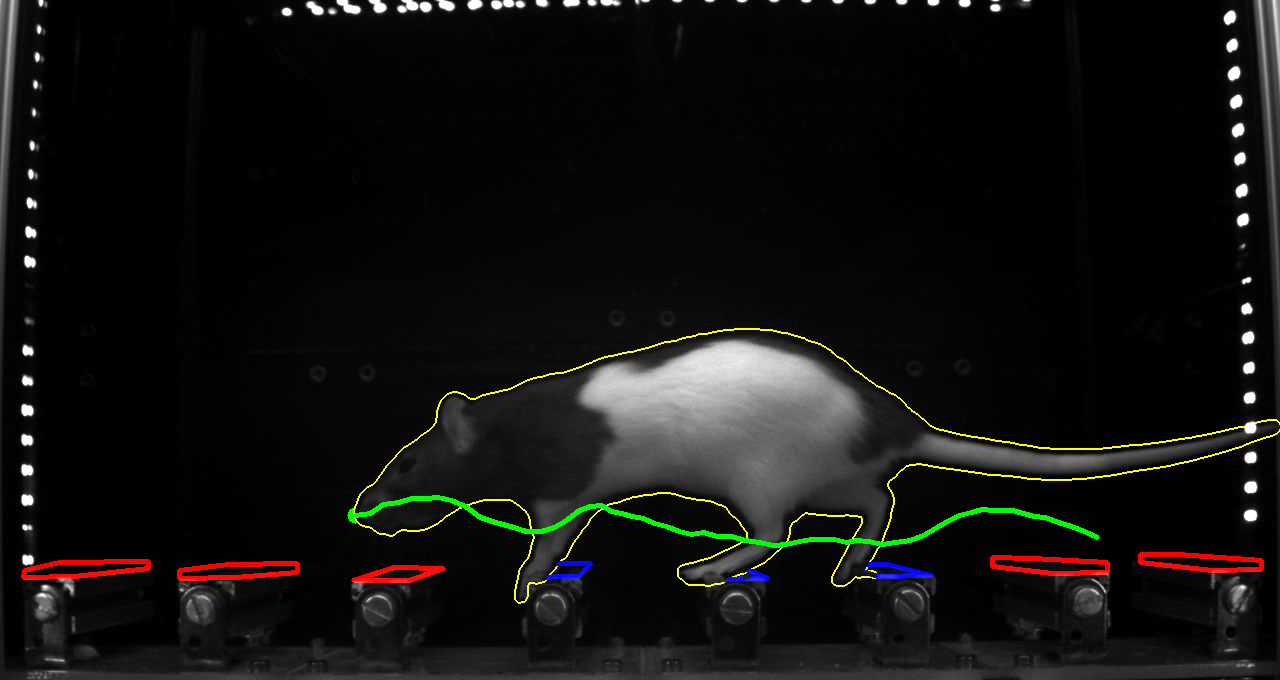
\includegraphics[width=0.75\columnwidth]{chapters/figuresChBehaviour/videography}
\end{center}
\vspace{-5mm}
\caption{Example video frame from the behaviour tracking system. Coloured overlays represent regions of interest and feature traces extracted automatically from the video.}
\label{fig:videography}
\end{figure}

Analysis routines were run using the NumPy scientific computing package \cite{Walt2011} and the Pandas data analysis library \cite{McKinney2010} for the Python programming language. Crossings were automatically extracted from the nose trajectory data by first detecting consecutive time points where the nose was positively identified in the video. In order for these periods to be successfully marked as crossings, the starting position of the nose must be located on the opposite side of the ending position. Inside each crossing, the moment of stepping with the forelimb on the centre steps was extracted by looking at the first peak above a threshold in the first derivative of the activation signal in the corresponding region of interest. False positive classifications due to hindlimb or tail activations were eliminated by enforcing the constraint that the position of the head must be located before the next step. Visual confirmation of the classified timepoints showed that spurious activations were all but eliminated by this procedure as stepping with the hindlimb or tail requires the head to be further ahead in space unless the animal turned around (in which case the trajectory would not be marked as a crossing anyway). The position of the nose at the moment of each step was extracted and found to be normally distributed, so statistical analysis of the step posture in the random condition used an unpaired t-test to check for independence of different measurement groups.

In order to evaluate the dynamics of crossing in the random condition, we first measured for every trial the speed at which the animals were moving on each spatial segment of the assay. To minimize overall trial-by-trial variation in individual animal performance, we used the average speed at which the animal approached the manipulated step as a baseline and subtracted it from the speed at each individual segment. To summarize differences in performance between stable and unstable trials, we then computed the average speed profile for each condition, and then subtracted the average speed profile for unstable trials from the average speed profile for stable trials. Finally, we computed the sum of all these speed differences at every segment in order to obtain the speedup index for each animal, i.e. an index of whether the animal tends to accelerate or decelerate across the assay on stable versus unstable trials.

\textbf{Video classification:} Classification of paw placement faults (i.e. slips) was performed in semi-automated fashion. First, possible slip timepoints were detected automatically using the peak detection method outlined above. All constraints on head position were relaxed for this analysis in order to exclude the possibility of false negatives. A human classifier then proceeded to manually go through each of the slip candidates and inspect the video around that timepoint in order to assess whether the activation peak was a genuine paw placement fault. Examples of false positives include tail and head activations as well as paw activations that occur while the animal is actively engaged in exploration, rearing, or other activities that are unrelated to crossing the obstacles.

Classification of behaviour responses following first exposure to the unstable condition was done on a frame-by-frame analysis of the high-speed video aligned on first contact with the manipulated step. The frame of first contact was defined as the first frame in which there is noticeable movement of the step caused by animal contact. Three main categories of behaviour were observed to follow the first contact: compensation, investigation and halting. Behaviour sequences were first classified as belonging to one of these categories and their onsets and offsets determined by the following criteria. Compensation behaviour is defined by a rapid and adaptive postural correction to the locomotion pattern in response to the perturbation. Onset of this behaviour is defined by the first frame in which there is visible rapid contraction of the body musculature following first contact. Investigation behaviour consists of periods of targeted interaction with the steps, often involving manipulation of the freely moving obstacle with the forepaws. The onset of this behaviour is defined by the animal orienting its head down to one of the manipulated steps, followed by subsequent interaction. Halting behaviour is characterized by a period in which the animal stops its ongoing motor program, and maintains the same body posture for several seconds, without switching to a new behaviour or orienting specifically to the manipulated steps. This behaviour is distinct from a freezing response, as occasional movements of the head are seen. Onset of this behaviour is defined by the moment where locomotion and other motor activities besides movement of the head come to a stop. A human classifier blind to the lesion condition was given descriptions of each of these three main categories of behaviour and asked to note onsets and offsets of each behaviour throughout the videos. These classifications provide a visual summary of the first response videos; the complete dataset used for this classification is included as supplementary movies.
